\documentclass{article}
\usepackage[T1]{fontenc}
\usepackage{color}
\usepackage{cite}
\usepackage[pdftex, bookmarks=true]{hyperref}
\usepackage{amsmath}
\usepackage{listings}
\usepackage{tikz}
\usepackage{pgfplots}

% Make a draft watermark.
% \usepackage{draftwatermark}
% \SetWatermarkFontSize{40pt}
% \SetWatermarkScale{4.0}

% TODO: Use bibtex or some better bibliography management
% tool.



% Define the speculative C++1y language.
\lstdefinelanguage{C++1y}{alsolanguage=C++,
                          escapechar=@,
                          breakatwhitespace=true,
                          morekeywords = {alignof, 
                                          decltype, 
                                          concept, 
                                          axiom, 
                                          requires, 
                                          property}}

% Program output
\lstdefinelanguage{Output}{}

% EBNF
\lstdefinelanguage{Ebnf}
{
  escapechar=@,
  basicstyle=\itshape\small
}


% Default formatting for listings.
%
% TODO: Define this as a style and make the code and program macros refer
% to the style.
\lstset{language=C++1y,
        basicstyle=\ttfamily\small,
        keywordstyle=\bfseries\color[rgb]{0,0,1},
        stringstyle=,
        xleftmargin=1em,
        showstringspaces=false,
        commentstyle=\rmfamily\itshape,
        columns=flexible,
        keepspaces=true,
        texcl=true}


%!TEX root = D0896.tex
% Definitions and redefinitions of special commands

%%--------------------------------------------------
%% Difference markups
\definecolor{addclr}{rgb}{0,.6,.6}
\definecolor{newclr}{rgb}{.6,.6,0}
\definecolor{oldclr}{rgb}{.6,0,.6}
\definecolor{newnewclr}{rgb}{.6,.6,0}
\definecolor{oldoldclr}{rgb}{.6,0,.6}
\definecolor{remclr}{rgb}{1,0,0}
\definecolor{noteclr}{rgb}{0,0,1}

\renewcommand{\added}[1]{\textcolor{addclr}{\uline{#1}}}
\newcommand{\removed}[1]{\textcolor{remclr}{\sout{#1}}}
\renewcommand{\changed}[2]{\removed{#1}\added{#2}}

% Mark-up text that is unique to the Ranges TS
% (\oldtxt{X} gets deleted in next draft, \newtxt{X} becomes \added{X}.)
\newcommand{\oldtxt}[1]{\textcolor{oldclr}{\sout{#1}}}
\newcommand{\newtxt}[1]{\textcolor{newclr}{\uline{#1}}}

% Mark-up text that is in the C++14 standard
% (\newnewtxt{X} becomes \added{X}.)
\newcommand{\newnewtxt}[1]{\newtxt{#1}}
% (\oldoldtxt{X} becomes \removed{X}.)
\newcommand{\oldoldtxt}[1]{\oldtxt{#1}}

\newcommand{\nbc}[1]{[#1]\ }
\newcommand{\addednb}[2]{\added{\nbc{#1}#2}}
\newcommand{\removednb}[2]{\removed{\nbc{#1}#2}}
\newcommand{\changednb}[3]{\removednb{#1}{#2}\added{#3}}
\newcommand{\remitem}[1]{\item\removed{#1}}

\newcommand{\ednote}[1]{\textcolor{noteclr}{[Editor's note: #1] }}
% \newcommand{\ednote}[1]{}

\newenvironment{addedblock}
{
\color{addclr}
}
{
\color{black}
}
\newenvironment{removedblock}
{
\color{remclr}
}
{
\color{black}
}

%%--------------------------------------------------
%% Sectioning macros.
% Each section has a depth, an automatically generated section
% number, a name, and a short tag.  The depth is an integer in
% the range [0,5].  (If it proves necessary, it wouldn't take much
% programming to raise the limit from 5 to something larger.)


% The basic sectioning command.  Example:
%    \Sec1[intro.scope]{Scope}
% defines a first-level section whose name is "Scope" and whose short
% tag is intro.scope.  The square brackets are mandatory.
\def\Sec#1[#2]#3{%
\ifcase#1\let\s=\chapter
      \or\let\s=\section
      \or\let\s=\subsection
      \or\let\s=\subsubsection
      \or\let\s=\paragraph
      \or\let\s=\subparagraph
      \fi%
\s[#3]{#3\hfill[#2]}\label{#2}}

% A convenience feature (mostly for the convenience of the Project
% Editor, to make it easy to move around large blocks of text):
% the \rSec macro is just like the \Sec macro, except that depths
% relative to a global variable, SectionDepthBase.  So, for example,
% if SectionDepthBase is 1,
%   \rSec1[temp.arg.type]{Template type arguments}
% is equivalent to
%   \Sec2[temp.arg.type]{Template type arguments}
\newcounter{SectionDepthBase}
\newcounter{scratch}

\def\rSec#1[#2]#3{%
\setcounter{scratch}{#1}
\addtocounter{scratch}{\value{SectionDepthBase}}
\Sec{\arabic{scratch}}[#2]{#3}}

\newcommand{\synopsis}[1]{\textbf{#1}}

%%--------------------------------------------------
% Indexing

% locations
\newcommand{\indextext}[1]{\index[generalindex]{#1}}
\newcommand{\indexlibrary}[1]{\index[libraryindex]{#1}}
\newcommand{\indexgram}[1]{\index[grammarindex]{#1}}
\newcommand{\indeximpldef}[1]{\index[impldefindex]{#1}}

\newcommand{\indexdefn}[1]{\indextext{#1}}
\newcommand{\indexgrammar}[1]{\indextext{#1}\indexgram{#1}}
\newcommand{\impldef}[1]{\indeximpldef{#1}implementation-defined}

% appearance
\newcommand{\idxcode}[1]{#1@\tcode{#1}}
\newcommand{\idxhdr}[1]{#1@\tcode{<#1>}}
\newcommand{\idxgram}[1]{#1@\textit{#1}}

%%--------------------------------------------------
% General code style
\newcommand{\CodeStyle}{\ttfamily}
\newcommand{\CodeStylex}[1]{\texttt{#1}}

% Code and definitions embedded in text.
\newcommand{\tcode}[1]{\CodeStylex{#1}}
\newcommand{\techterm}[1]{\textit{#1}\xspace}
\newcommand{\defnx}[2]{\indexdefn{#2}\textit{#1}\xspace}
\newcommand{\defn}[1]{\defnx{#1}{#1}}
\newcommand{\term}[1]{\textit{#1}\xspace}
\newcommand{\grammarterm}[1]{\textit{#1}\xspace}
\newcommand{\placeholder}[1]{\textit{#1}\xspace}
\newcommand{\libconcept}[1]{\CodeStylex{#1}}

%%--------------------------------------------------
%% allow line break if needed for justification
\newcommand{\brk}{\discretionary{}{}{}}
%  especially for scope qualifier
\newcommand{\colcol}{\brk::\brk}

%%--------------------------------------------------
%% Macros for funky text
\newcommand{\Rplus}{\protect\hspace{-.1em}\protect\raisebox{.35ex}{\smaller{\smaller\textbf{+}}}}
% \newcommand{\Rplus}{+}
\newcommand{\Cpp}{\mbox{C\Rplus\Rplus}\xspace}
\newcommand{\CppIII}{\Cpp 2003\xspace}
\newcommand{\CppXI}{\Cpp 2011\xspace}
\newcommand{\opt}{{\ensuremath{_\mathit{opt}}}\xspace}
\newcommand{\shl}{<{<}}
\newcommand{\shr}{>{>}}
\newcommand{\dcr}{-{-}}
\newcommand{\exor}{\^{}}
\newcommand{\bigoh}[1]{\ensuremath{\mathscr{O}(#1)}}

% Make all tildes a little larger to avoid visual similarity with hyphens.
% FIXME: Remove \tilde in favour of \~.
%\renewcommand{\tilde}{\textasciitilde}
%\renewcommand{\~}{\textasciitilde}
%\let\OldTextAsciiTilde\textasciitilde
%\renewcommand{\textasciitilde}{\protect\raisebox{-0.17ex}{\larger\OldTextAsciiTilde}}

%%--------------------------------------------------
%% States and operators
\newcommand{\state}[2]{\tcode{#1}\ensuremath{_{#2}}}
\newcommand{\bitand}{\ensuremath{\, \mathsf{bitand} \,}}
\newcommand{\bitor}{\ensuremath{\, \mathsf{bitor} \,}}
\newcommand{\xor}{\ensuremath{\, \mathsf{xor} \,}}
\newcommand{\rightshift}{\ensuremath{\, \mathsf{rshift} \,}}
\newcommand{\leftshift}[1]{\ensuremath{\, \mathsf{lshift}_#1 \,}}

%% Notes and examples
\newcommand{\EnterBlock}[1]{[\,\textit{#1:}\xspace}
\newcommand{\ExitBlock}[1]{\textit{\,---\,end #1}\,]\xspace}
\newcommand{\enternote}{\EnterBlock{Note}}
\newcommand{\exitnote}{\ExitBlock{note}}
\newcommand{\enterexample}{\EnterBlock{Example}}
\newcommand{\exitexample}{\ExitBlock{example}}

%% Library function descriptions
\newcommand{\Fundescx}[1]{\textit{#1}\xspace}
\newcommand{\Fundesc}[1]{\Fundescx{#1:}}
\newcommand{\required}{\Fundesc{Required behavior}}
\newcommand{\requires}{\Fundesc{Requires}}
\newcommand{\constraints}{\Fundesc{Constraints}}
\newcommand{\mandates}{\Fundesc{Mandates}}
\newcommand{\expects}{\Fundesc{Expects}}
\newcommand{\effects}{\Fundesc{Effects}}
\newcommand{\ensures}{\Fundesc{Ensures}}
\newcommand{\returns}{\Fundesc{Returns}}
\newcommand{\throws}{\Fundesc{Throws}}
\newcommand{\default}{\Fundesc{Default behavior}}
\newcommand{\complexity}{\Fundesc{Complexity}}
\newcommand{\remark}{\Fundesc{Remark}}
\newcommand{\remarks}{\Fundesc{Remarks}}
\newcommand{\noteintro}[1]{[\textit{#1}:\space}
\newcommand{\noteoutro}[1]{\textit{\,---\,end #1}\kern.5pt]}
\newenvironment{note}[1][Note]{\noteintro{#1}}{\noteoutro{note}\space}
\newenvironment{example}[1][Example]{\noteintro{#1}}{\noteoutro{example}\space}
\newcommand{\realnote}{\Fundesc{Note}}
\newcommand{\realnotes}{\Fundesc{Notes}}
\newcommand{\errors}{\Fundesc{Error conditions}}
\newcommand{\sync}{\Fundesc{Synchronization}}
\newcommand{\implimits}{\Fundesc{Implementation limits}}
\newcommand{\replaceable}{\Fundesc{Replaceable}}
\newcommand{\exceptionsafety}{\Fundesc{Exception safety}}
\newcommand{\returntype}{\Fundesc{Return type}}
\newcommand{\cvalue}{\Fundesc{Value}}
\newcommand{\ctype}{\Fundesc{Type}}
\newcommand{\ctypes}{\Fundesc{Types}}
\newcommand{\dtype}{\Fundesc{Default type}}
\newcommand{\ctemplate}{\Fundesc{Class template}}
\newcommand{\templalias}{\Fundesc{Alias template}}

%% Cross reference
\newcommand{\xref}{\textsc{See also:}\xspace}
\newcommand{\xsee}{\textsc{See:}\xspace}

%% NTBS, etc.
\newcommand{\NTS}[1]{\textsc{#1}\xspace}
\newcommand{\ntbs}{\NTS{ntbs}}
\newcommand{\ntmbs}{\NTS{ntmbs}}
\newcommand{\ntwcs}{\NTS{ntwcs}}
\newcommand{\ntcxvis}{\NTS{ntc16s}}
\newcommand{\ntcxxxiis}{\NTS{ntc32s}}

%% Code annotations
\newcommand{\EXPO}[1]{\textit{#1}}
\newcommand{\expos}{\EXPO{exposition only}}
\newcommand{\impdef}{\EXPO{implementation-defined}}
\newcommand{\impdefx}[1]{\indeximpldef{#1}\EXPO{implementation-defined}}
\newcommand{\notdef}{\EXPO{not defined}}

\newcommand{\UNSP}[1]{\textit{\texttt{#1}}}
\newcommand{\unspec}{\UNSP{unspecified}\xspace}
\newcommand{\unspecbool}{\UNSP{unspecified-bool-type}}
\newcommand{\seebelow}{\UNSP{see below}}
\newcommand{\unspecuniqtype}{\UNSP{unspecified unique type}}
\newcommand{\unspecalloctype}{\UNSP{unspecified allocator type}}

%% Double underscore
\newcommand{\ungap}{\kern.5pt}
\newcommand{\unun}{\_\ungap\_}
\newcommand{\xname}[1]{\texorpdfstring{\unun\ungap#1}{\_\_#1}}
\newcommand{\mname}[1]{\tcode{\unun\ungap#1\ungap\unun}}

%% Ranges
\newcommand{\Range}[4]{\tcode{#1\brk{}#3,\brk{}#4\brk{}#2}\xspace}
\newcommand{\crange}[2]{\Range{[}{]}{#1}{#2}}
\newcommand{\brange}[2]{\Range{(}{]}{#1}{#2}}
\newcommand{\orange}[2]{\Range{(}{)}{#1}{#2}}
\newcommand{\range}[2]{\Range{[}{)}{#1}{#2}}

%% Change descriptions
\newcommand{\diffdef}[1]{\hfill\break\textbf{#1:}\xspace}
\newcommand{\change}{\diffdef{Change}}
\newcommand{\rationale}{\diffdef{Rationale}}
\newcommand{\effect}{\diffdef{Effect on original feature}}
\newcommand{\difficulty}{\diffdef{Difficulty of converting}}
\newcommand{\howwide}{\diffdef{How widely used}}

%% Miscellaneous
\newcommand{\uniquens}{\textrm{\textit{\textbf{unique}}} }
\newcommand{\stage}[1]{\item{\textbf{Stage #1:}}\xspace}
\newcommand{\doccite}[1]{\textit{#1}\xspace}
\newcommand{\cvqual}[1]{\textit{#1}}
\newcommand{\cv}{\cvqual{cv}}
\renewcommand{\emph}[1]{\textit{#1}\xspace}
\newcommand{\numconst}[1]{\textsl{#1}\xspace}
\newcommand{\logop}[1]{{\footnotesize #1}\xspace}

%%--------------------------------------------------
%% Environments for code listings.

% We use the 'listings' package, with some small customizations.  The
% most interesting customization: all TeX commands are available
% within comments.  Comments are set in italics, keywords and strings
% don't get special treatment.

\lstset{language=C++,
        basicstyle=\small\CodeStyle,
        keywordstyle=,
        stringstyle=,
        xleftmargin=1em,
        showstringspaces=false,
        commentstyle=\itshape\rmfamily,
        columns=flexible,
        keepspaces=true,
        texcl=true}

% Our usual abbreviation for 'listings'.  Comments are in
% italics.  Arbitrary TeX commands can be used if they're
% surrounded by @ signs.
\newcommand{\CodeBlockSetup}{
 \lstset{escapechar=@}
 \renewcommand{\tcode}[1]{\textup{\CodeStylex{##1}}}
 \renewcommand{\techterm}[1]{\textit{\CodeStylex{##1}}}
 \renewcommand{\term}[1]{\textit{##1}}
 \renewcommand{\grammarterm}[1]{\textit{##1}}
}
\lstnewenvironment{codeblock}{\CodeBlockSetup}{}

% A code block in which single-quotes are digit separators
% rather than character literals.
\lstnewenvironment{codeblockdigitsep}{
 \CodeBlockSetup
 \lstset{deletestring=[b]{'}}
}{}

% Permit use of '@' inside codeblock blocks (don't ask)
\makeatletter
\newcommand{\atsign}{@}
\makeatother

%%--------------------------------------------------
%% Indented text
\newenvironment{indented}
{\list{}{}\item\relax}
{\endlist}

%%--------------------------------------------------
%% Library item descriptions
\lstnewenvironment{itemdecl}
{
 \lstset{escapechar=@,
 xleftmargin=0em,
 aboveskip=2ex,
 belowskip=0ex	% leave this alone: it keeps these things out of the
				% footnote area
 }
}
{
}

\newenvironment{itemdescr}
{
 \begin{indented}}
{
 \end{indented}
}


%%--------------------------------------------------
%% Bnf environments
\newlength{\BnfIndent}
\setlength{\BnfIndent}{\leftmargini}
\newlength{\BnfInc}
\setlength{\BnfInc}{\BnfIndent}
\newlength{\BnfRest}
\setlength{\BnfRest}{2\BnfIndent}
\newcommand{\BnfNontermshape}{\small\rmfamily\itshape}
\newcommand{\BnfTermshape}{\small\ttfamily\upshape}
\newcommand{\nonterminal}[1]{{\BnfNontermshape #1}}

\newenvironment{bnfbase}
 {
 \newcommand{\nontermdef}[1]{\nonterminal{##1}\indexgrammar{\idxgram{##1}}:}
 \newcommand{\terminal}[1]{{\BnfTermshape ##1}\xspace}
 \newcommand{\descr}[1]{\normalfont{##1}}
 \newcommand{\bnfindentfirst}{\BnfIndent}
 \newcommand{\bnfindentinc}{\BnfInc}
 \newcommand{\bnfindentrest}{\BnfRest}
 \begin{minipage}{.9\hsize}
 \newcommand{\br}{\hfill\\}
 \frenchspacing
 }
 {
 \nonfrenchspacing
 \end{minipage}
 }

\newenvironment{BnfTabBase}[1]
{
 \begin{bnfbase}
 #1
 \begin{indented}
 \begin{tabbing}
 \hspace*{\bnfindentfirst}\=\hspace{\bnfindentinc}\=\hspace{.6in}\=\hspace{.6in}\=\hspace{.6in}\=\hspace{.6in}\=\hspace{.6in}\=\hspace{.6in}\=\hspace{.6in}\=\hspace{.6in}\=\hspace{.6in}\=\hspace{.6in}\=\kill}
{
 \end{tabbing}
 \end{indented}
 \end{bnfbase}
}

\newenvironment{bnfkeywordtab}
{
 \begin{BnfTabBase}{\BnfTermshape}
}
{
 \end{BnfTabBase}
}

\newenvironment{bnftab}
{
 \begin{BnfTabBase}{\BnfNontermshape}
}
{
 \end{BnfTabBase}
}

\newenvironment{simplebnf}
{
 \begin{bnfbase}
 \BnfNontermshape
 \begin{indented}
}
{
 \end{indented}
 \end{bnfbase}
}

\newenvironment{bnf}
{
 \begin{bnfbase}
 \list{}
	{
	\setlength{\leftmargin}{\bnfindentrest}
	\setlength{\listparindent}{-\bnfindentinc}
	\setlength{\itemindent}{\listparindent}
	}
 \BnfNontermshape
 \item\relax
}
{
 \endlist
 \end{bnfbase}
}

% non-copied versions of bnf environments
\newenvironment{ncbnftab}
{
 \begin{bnftab}
}
{
 \end{bnftab}
}

\newenvironment{ncsimplebnf}
{
 \begin{simplebnf}
}
{
 \end{simplebnf}
}

\newenvironment{ncbnf}
{
 \begin{bnf}
}
{
 \end{bnf}
}

%%--------------------------------------------------
%% Drawing environment
%
% usage: \begin{drawing}{UNITLENGTH}{WIDTH}{HEIGHT}{CAPTION}
\newenvironment{drawing}[4]
{
\newcommand{\mycaption}{#4}
\begin{figure}[h]
\setlength{\unitlength}{#1}
\begin{center}
\begin{picture}(#2,#3)\thicklines
}
{
\end{picture}
\end{center}
\caption{\mycaption}
\end{figure}
}

%%--------------------------------------------------
%% Environment for imported graphics
% usage: \begin{importgraphic}{CAPTION}{TAG}{FILE}

\newenvironment{importgraphic}[3]
{%
\newcommand{\cptn}{#1}
\newcommand{\lbl}{#2}
\begin{figure}[htp]\centering%
\includegraphics[scale=.35]{#3}
}
{
\caption{\cptn}\label{\lbl}%
\end{figure}}

%% enumeration display overrides
% enumerate with lowercase letters
\newenvironment{enumeratea}
{
 \renewcommand{\labelenumi}{\alph{enumi})}
 \begin{enumerate}
}
{
 \end{enumerate}
}

% enumerate with arabic numbers
\newenvironment{enumeraten}
{
 \renewcommand{\labelenumi}{\arabic{enumi})}
 \begin{enumerate}
}
{
 \end{enumerate}
}

%%--------------------------------------------------
%% Cross references.
\newcommand{\addxref}[1]{\glossary[xrefindex]{#1}{(\ref{#1})}}

%%--------------------------------------------------
%% Definitions section
% usage: \definition{name}{xref}
%\newcommand{\definition}[2]{\rSec2[#2]{#1}}
% for ISO format, use:
\newcommand{\definition}[2]
 {\hfill\vspace{.25ex plus .5ex minus .2ex}\\
 \addtocounter{subsection}{1}%
 \textbf{\thesubsection\hfill\relax[#2]}\\
 \textbf{#1}\label{#2}\\
 }

%%--------------------------------------------------
%% Definitions section for "Terms and definitions"
\newcommand{\nocontentsline}[3]{}
\newcommand{\definitionx}[3]{%
\addxref{#3}%
\let\oldcontentsline\addcontentsline%
\let\addcontentsline\nocontentsline%
#1[#2]{\hfill[#3]}\vspace{-.3\onelineskip}\label{#3} \textbf{#2}\\*%
\let\addcontentsline\oldcontentsline%
}
\newcommand{\defncontext}[1]{\textlangle#1\textrangle}


\begin{document}

\noindent\textbf{Document Number:} D0429R0\\
\textbf{Date:} 2016-08-31\\
\textbf{Reply to:} whatwasthataddress@gmail.com\\
\textbf{Audience:} LWG/LEWG

\title{\textbf{\Large A Standard \code{flat_map}}}
\author{
  \makebox[.25\linewidth]{T. Zachary Laine}\\NVIDIA\\
}
\date{}
{\let\newpage\relax\maketitle}


\section{Introduction}

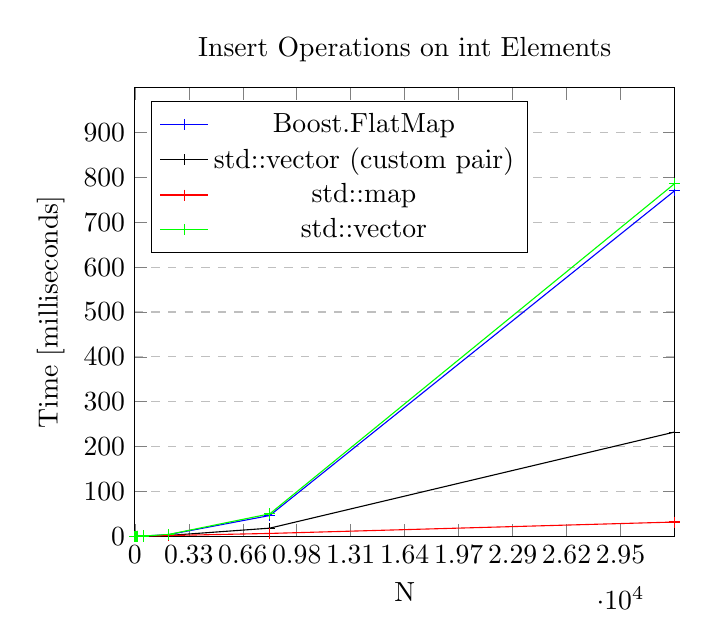
\begin{tikzpicture}
    \begin{axis}[
        title={Insert Operations on int Elements},
        xlabel={N},
        ylabel={Time [milliseconds]},
        xmin=0, xmax=32768.0,
        ymin=0, ymax=1000.0,
        xtick={0.0,3276.8,6553.6,9830.4,13107.2,16384.0,19660.8,22937.6,26214.4,29491.2},
        ytick={0.0,100.0,200.0,300.0,400.0,500.0,600.0,700.0,800.0,900.0},
        legend pos=north west,
        ymajorgrids=true,
        grid style=dashed,
        legend entries={Boost.FlatMap,std::vector (custom pair),std::map,std::vector}
        ]

    \addplot[color=blue,mark=+,]
        coordinates {(8,0.0061)(32,0.009)(128,0.0466)(512,0.3269)(2048,3.4296)(8192,46.1462)(32768,770.289)};

    \addplot[color=black,mark=+,]
        coordinates {(8,0.0051)(32,0.0133)(128,0.1292)(512,0.2641)(2048,1.6346)(8192,17.9527)(32768,232.288)};

    \addplot[color=red,mark=+,]
        coordinates {(8,0.0084)(32,0.0187)(128,0.0794)(512,0.3573)(2048,1.4816)(8192,6.1507)(32768,31.5773)};

    \addplot[color=green,mark=+,]
        coordinates {(8,0.0045)(32,0.0135)(128,0.0535)(512,0.3669)(2048,3.8914)(8192,49.8729)(32768,786.225)};

    \end{axis}
\end{tikzpicture}


\label{sec:intro}

This paper outlines what a (mostly) API-compatible, non-node-based \code{map}
might look like.  Rather than presenting a final design, this paper is
intended as a starting point for discussion and as a basis for future work.
Specifically, there is no mention of \code{multimap}, \code{set}, or
\code{multiset}.  Those will be added in later papers.

\section{Motivation and Scope}

There has been a strong desire for a more space- and/or runtime-efficient
representation for \code{map} among C++ users for some time now.  This has
motivated discussions among the members of SG14 resulting in a
paper\footnote{See P0038R0,
  \href{http://www.open-std.org/jtc1/sc22/wg21/docs/papers/2015/p0038r0.html}{here}.},
numerous articles and talks, and an implementation in Boost,
\code{boost::container::flat_map}\footnote{Part of Boost.Container,
  \href{http://www.boost.org/doc/libs/1_61_0/doc/html/container.html}{here}.}.
Virtually everyone who makes games, embedded, or system software in C++ uses
the Boost implementation or one that they rolled themselves.\\

Here are some numbers that show why.  The graphs that follow show runtimes for
different \code{map}-like associative containers.  The containers used are
Boost.FlatMap, \code{map}, and two thin wrappers over a sorted \code{vector};
the ``custom pair'' version of the sorted \code{vector} uses a simple
\code{struct} instead of \code{pair} for its value type.  All containers use
an \code{int} as the key type and an \code{int} or a \code{struct} with 5
\code{double}s for the value type.\\

All the graphs below were produced on Windows with MSVC 2015.  Similar results
were obtained on Linux, with Clang 3.9 and libc++, and with g++ 4.8.4 and
libstdc++.\\

These four TODO graphs cover the \code{int}-value-type case.  The first graph
shows insertion of N elements with random keys; the second shows full
iteration across all N elements; the third shows \code{map.find()} called once
for each key used in the original insertions; and the fourth shows erasure of
all N elements, by the keys used in the original insertions.

\begin{tikzpicture}[baseline]
    \begin{groupplot}[group style={group size= 2 by 4}, width=3.25in]

    \nextgroupplot[
        %small,%legend pos=outer north east,legend entries={Boost.FlatMap,std::map,std::unordered\_map,std::vector,std::vector (custom pair)},
        %width=3.75in,
        title={Insert Operations, <int, int> Elements},
        xlabel={N},
        ylabel=\empty,%{Time [milliseconds]},
        xmin=0, xmax=10000,
        ymin=0, ymax=30.0,
        xtick={10,100,1000,10000,100000},
        xticklabels={10,,$10^{3}$,$10^{4}$,$10^{5}$},
        ytick={0.0,10.0,20.0,30.0,40.0},
        ymajorgrids=true,
        grid style=dashed,
        scaled x ticks=false,
        scaled y ticks=true,
        ]

    \addplot[color=blue,mark=|,no markers,]
        coordinates {(10,0.007626)(100,0.0725654)(1000,0.748165)(10000,25.2264)};

    \addplot[color=red,mark=|,no markers,]
        coordinates {(10,0.0070264)(100,0.0703298)(1000,0.612005)(10000,6.07091)};

    \addplot[color=brown,mark=|,no markers,]
        coordinates {(10,0.0082692)(100,0.0839602)(1000,0.65392)(10000,6.22599)};

    \addplot[color=green,mark=|,no markers,]
        coordinates {(10,0.0069982)(100,0.0640582)(1000,0.750933)(10000,23.9862)};

    \addplot[color=black,mark=|,no markers,]
        coordinates {(10,0.006927)(100,0.0595058)(1000,0.628059)(10000,11.1191)};

    \coordinate (top) at (rel axis cs:0,1);% coordinate at top of the first plot

    \nextgroupplot[
        %small,
        %width=3.75in,
        title={Insert Operations, <string, string> Elements},
        xlabel={N},
        ylabel=\empty,%{Time [milliseconds]},
        xmin=0, xmax=10000,
        ymin=0, ymax=400.0,
        xtick={10,100,1000,10000,100000},
        xticklabels={10,,$10^{3}$,$10^{4}$,$10^{5}$},
        ytick={0.0,100.0,200.0,300.0,400.0,500.0},
        ymajorgrids=true,
        grid style=dashed,
        scaled x ticks=false,
        scaled y ticks=true,
        ]

    \addplot[color=blue,mark=|,no markers,]
        coordinates {(10,0.0070676)(100,0.0932798)(1000,4.41807)(10000,293.533)};
    \label{plots:plot1}

    \addplot[color=red,mark=|,no markers,]
        coordinates {(10,0.0065504)(100,0.0683816)(1000,0.777764)(10000,8.74438)};
    \label{plots:plot2}

    \addplot[color=brown,mark=|,no markers,]
        coordinates {(10,0.007151)(100,0.0716148)(1000,0.740306)(10000,7.42573)};
    \label{plots:plot3}

    \addplot[color=green,mark=|,no markers,]
        coordinates {(10,0.0071808)(100,0.0908476)(1000,4.43712)(10000,302.252)};
    \label{plots:plot4}

    \addplot[color=black,mark=|,no markers,]
        coordinates {(10,0.007098)(100,0.0902228)(1000,4.43289)(10000,286.363)};
    \label{plots:plot5}

    \coordinate (bot) at (rel axis cs:1,0);% coordinate at bottom of the last plot

    \end{groupplot}%
    \path (top-|current bounding box.west)-- 
          node[anchor=south,rotate=90] {Time [milliseconds]} 
          (bot-|current bounding box.west);

% legend
\path (top|-current bounding box.south)--
      coordinate(legendpos)
      (bot|-current bounding box.south);
\matrix[
    matrix of nodes,
    anchor=south,
    draw,
    inner sep=0.2em,
    draw
  ]at([yshift=-5ex]legendpos)
  {
    \ref{plots:plot1}& Boost.FlatMap&[5pt]
    \ref{plots:plot2}& std::map&[5pt]
    \ref{plots:plot3}& std::unordered\_map&[5pt]
    \ref{plots:plot4}& std::vector&[5pt]
    \ref{plots:plot5}& std::vector (custom pair)&[5pt]\\
  };
\end{tikzpicture}
\\
\\

As one might expect, insertionion takes longer in contiguous-storage
implementations.  Boost.FlatMap and a sorted \code{vector<pair<int, int>>}
have superlinear growth in insertion time.  While the curve for sorted
\code{vector} using a custom \code{struct} instead of a \code{pair} is
superlinear as well, it is dramatically flatter in its growth -- much closer
to node-based \code{map}.

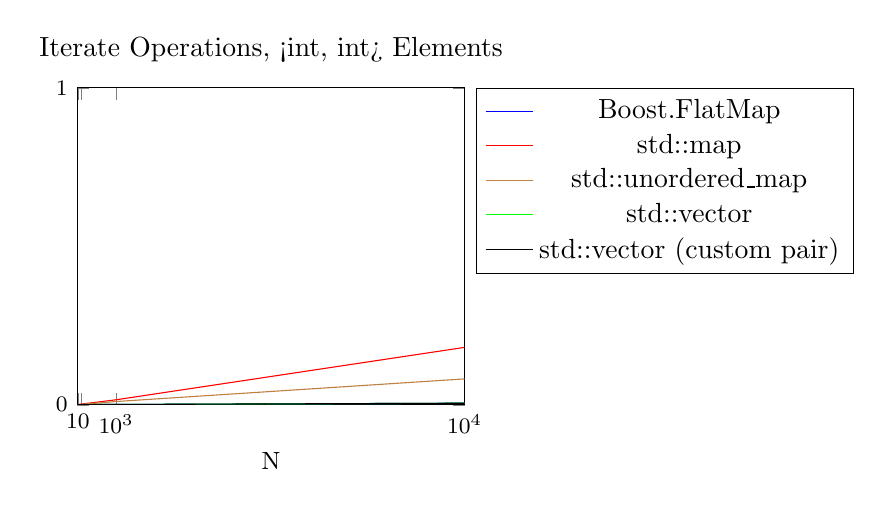
\begin{tikzpicture}[baseline]
    \begin{axis}[
        small,legend pos=outer north east,legend entries={Boost.FlatMap,std::map,std::unordered\_map,std::vector,std::vector (custom pair)},
        %width=3.75in,
        title={Iterate Operations, <int, int> Elements},
        xlabel={N},
        ylabel=\empty,%{Time [milliseconds]},
        xmin=0, xmax=10000,
        ymin=0, ymax=1.0,
        xtick={10,100,1000,10000,100000},
        xticklabels={10,,$10^{3}$,$10^{4}$,$10^{5}$},
        ytick={0.0,1.0,2.0},
        ymajorgrids=true,
        grid style=dashed,
        scaled x ticks=false,
        scaled y ticks=true,
        ]

    \addplot[color=blue,mark=|,no markers,]
        coordinates {(10,0.0006148)(100,0.0007682)(1000,0.000978)(10000,0.0049866)};

    \addplot[color=red,mark=|,no markers,]
        coordinates {(10,0.0007122)(100,0.002165)(1000,0.015826)(10000,0.181238)};

    \addplot[color=brown,mark=|,no markers,]
        coordinates {(10,0.0007266)(100,0.001299)(1000,0.0102944)(10000,0.0817004)};

    \addplot[color=green,mark=|,no markers,]
        coordinates {(10,0.0007266)(100,0.0006282)(1000,0.000978)(10000,0.0049446)};

    \addplot[color=black,mark=|,no markers,]
        coordinates {(10,0.0006286)(100,0.0006148)(1000,0.000964)(10000,0.0049028)};

    \end{axis}%
\end{tikzpicture}%
~%
%
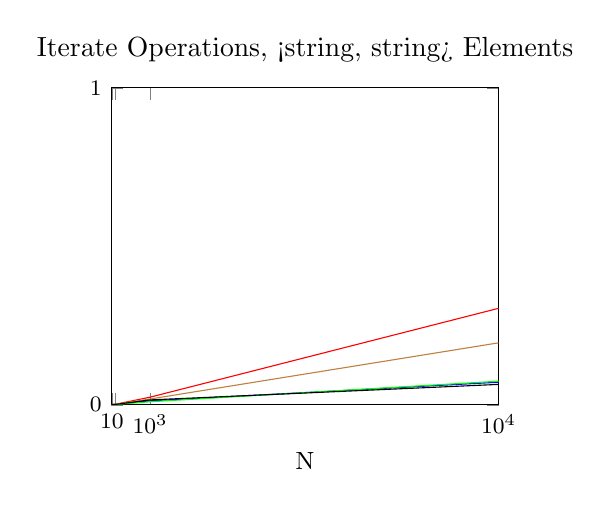
\begin{tikzpicture}[baseline]
    \begin{axis}[
        small,
        %width=3.75in,
        title={Iterate Operations, <string, string> Elements},
        xlabel={N},
        ylabel=\empty,%{Time [milliseconds]},
        xmin=0, xmax=10000,
        ymin=0, ymax=1.0,
        xtick={10,100,1000,10000,100000},
        xticklabels={10,,$10^{3}$,$10^{4}$,$10^{5}$},
        ytick={0.0,1.0,2.0},
        ymajorgrids=true,
        grid style=dashed,
        scaled x ticks=false,
        scaled y ticks=true,
        ]

    \addplot[color=blue,mark=|,no markers,]
        coordinates {(10,0.0007126)(100,0.0011034)(1000,0.0124458)(10000,0.0711818)};

    \addplot[color=red,mark=|,no markers,]
        coordinates {(10,0.0007268)(100,0.0015926)(1000,0.0240674)(10000,0.304508)};

    \addplot[color=brown,mark=|,no markers,]
        coordinates {(10,0.000629)(100,0.0012296)(1000,0.0182844)(10000,0.195542)};

    \addplot[color=green,mark=|,no markers,]
        coordinates {(10,0.0007262)(100,0.0011312)(1000,0.0095966)(10000,0.074521)};

    \addplot[color=black,mark=|,no markers,]
        coordinates {(10,0.0006708)(100,0.001118)(1000,0.0153788)(10000,0.0643378)};

    \end{axis}%
\end{tikzpicture}%
~%
%

For all variants but \code{map}, iteration is relatively similar, and much
faster that \code{map}'s.

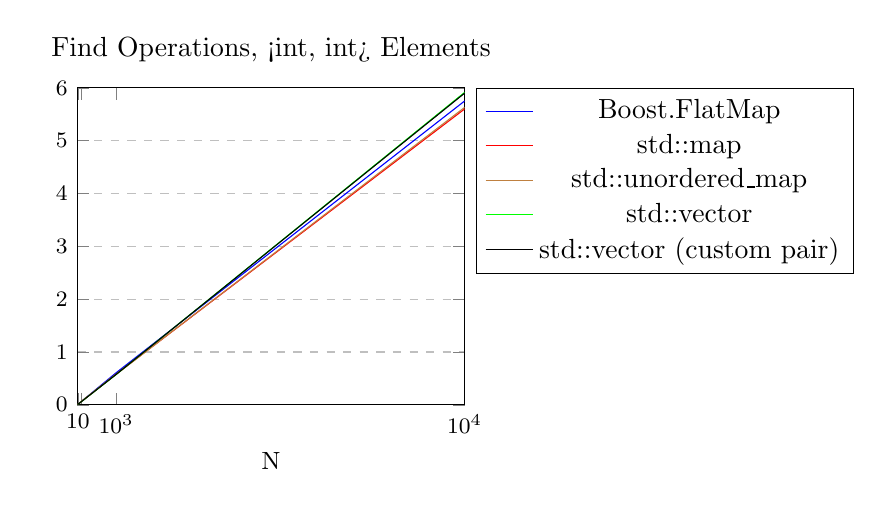
\begin{tikzpicture}[baseline]
    \begin{axis}[
        small,legend pos=outer north east,legend entries={Boost.FlatMap,std::map,std::unordered\_map,std::vector,std::vector (custom pair)},
        %width=3.75in,
        title={Find Operations, <int, int> Elements},
        xlabel={N},
        ylabel=\empty,%{Time [milliseconds]},
        xmin=0, xmax=10000,
        ymin=0, ymax=6.0,
        xtick={10,100,1000,10000,100000},
        xticklabels={10,,$10^{3}$,$10^{4}$,$10^{5}$},
        ytick={0.0,1.0,2.0,3.0,4.0,5.0,6.0,7.0},
        ymajorgrids=true,
        grid style=dashed,
        scaled x ticks=false,
        scaled y ticks=true,
        ]

    \addplot[color=blue,mark=|,no markers,]
        coordinates {(10,0.0061042)(100,0.0619778)(1000,0.60702)(10000,5.75315)};

    \addplot[color=red,mark=|,no markers,]
        coordinates {(10,0.0065656)(100,0.0617254)(1000,0.580172)(10000,5.60213)};

    \addplot[color=brown,mark=|,no markers,]
        coordinates {(10,0.0064952)(100,0.0629964)(1000,0.576962)(10000,5.63177)};

    \addplot[color=green,mark=|,no markers,]
        coordinates {(10,0.0063698)(100,0.0582888)(1000,0.573966)(10000,5.91615)};

    \addplot[color=black,mark=|,no markers,]
        coordinates {(10,0.0064248)(100,0.0581646)(1000,0.575594)(10000,5.90158)};

    \end{axis}%
\end{tikzpicture}%
~%
%
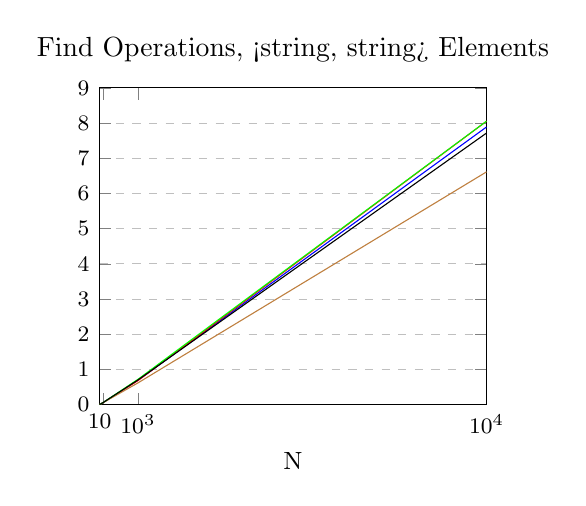
\begin{tikzpicture}[baseline]
    \begin{axis}[
        small,
        %width=3.75in,
        title={Find Operations, <string, string> Elements},
        xlabel={N},
        ylabel=\empty,%{Time [milliseconds]},
        xmin=0, xmax=10000,
        ymin=0, ymax=9.0,
        xtick={10,100,1000,10000,100000},
        xticklabels={10,,$10^{3}$,$10^{4}$,$10^{5}$},
        ytick={0.0,1.0,2.0,3.0,4.0,5.0,6.0,7.0,8.0,9.0,10.0},
        ymajorgrids=true,
        grid style=dashed,
        scaled x ticks=false,
        scaled y ticks=true,
        ]

    \addplot[color=blue,mark=|,no markers,]
        coordinates {(10,0.006118)(100,0.062631)(1000,0.695828)(10000,7.89026)};

    \addplot[color=red,mark=|,no markers,]
        coordinates {(10,0.006146)(100,0.061546)(1000,0.687874)(10000,8.05409)};

    \addplot[color=brown,mark=|,no markers,]
        coordinates {(10,0.0062576)(100,0.060553)(1000,0.621572)(10000,6.61517)};

    \addplot[color=green,mark=|,no markers,]
        coordinates {(10,0.0065508)(100,0.0637798)(1000,0.723151)(10000,8.05563)};

    \addplot[color=black,mark=|,no markers,]
        coordinates {(10,0.0064962)(100,0.063536)(1000,0.705945)(10000,7.71759)};

    \end{axis}%
\end{tikzpicture}%
~%
%

\code{find()} performance is roughly similar across all the
implementations, and they all show superlinear growth.  Note that
Boost.FlatMap performs the best here.

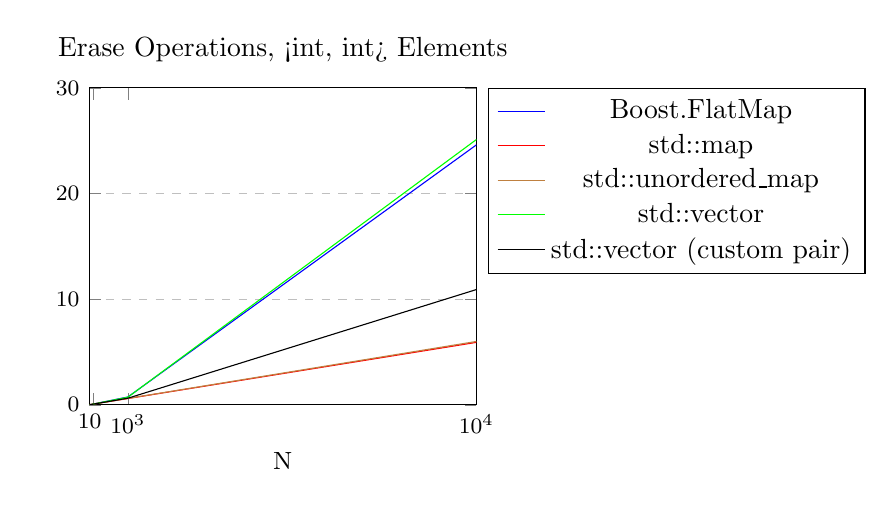
\begin{tikzpicture}[baseline]
    \begin{axis}[
        small,legend pos=outer north east,legend entries={Boost.FlatMap,std::map,std::unordered\_map,std::vector,std::vector (custom pair)},
        %width=3.75in,
        title={Erase Operations, <int, int> Elements},
        xlabel={N},
        ylabel=\empty,%{Time [milliseconds]},
        xmin=0, xmax=10000,
        ymin=0, ymax=30.0,
        xtick={10,100,1000,10000,100000},
        xticklabels={10,,$10^{3}$,$10^{4}$,$10^{5}$},
        ytick={0.0,10.0,20.0,30.0,40.0},
        ymajorgrids=true,
        grid style=dashed,
        scaled x ticks=false,
        scaled y ticks=true,
        ]

    \addplot[color=blue,mark=|,no markers,]
        coordinates {(10,0.0064952)(100,0.0667284)(1000,0.738798)(10000,24.6091)};

    \addplot[color=red,mark=|,no markers,]
        coordinates {(10,0.006774)(100,0.0651334)(1000,0.591387)(10000,5.90963)};

    \addplot[color=brown,mark=|,no markers,]
        coordinates {(10,0.0072904)(100,0.0710708)(1000,0.604785)(10000,5.99803)};

    \addplot[color=green,mark=|,no markers,]
        coordinates {(10,0.0067054)(100,0.0593234)(1000,0.724238)(10000,25.1154)};

    \addplot[color=black,mark=|,no markers,]
        coordinates {(10,0.0065508)(100,0.058947)(1000,0.624071)(10000,10.9113)};

    \end{axis}%
\end{tikzpicture}%
~%
%
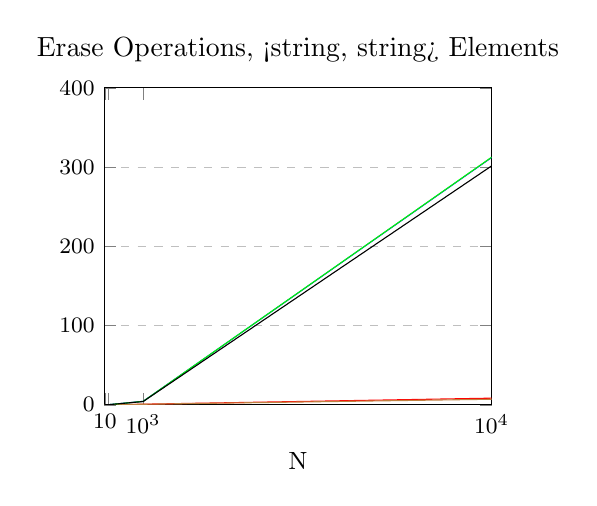
\begin{tikzpicture}[baseline]
    \begin{axis}[
        small,
        %width=3.75in,
        title={Erase Operations, <string, string> Elements},
        xlabel={N},
        ylabel=\empty,%{Time [milliseconds]},
        xmin=0, xmax=10000,
        ymin=0, ymax=400.0,
        xtick={10,100,1000,10000,100000},
        xticklabels={10,,$10^{3}$,$10^{4}$,$10^{5}$},
        ytick={0.0,100.0,200.0,300.0,400.0,500.0},
        ymajorgrids=true,
        grid style=dashed,
        scaled x ticks=false,
        scaled y ticks=true,
        ]

    \addplot[color=blue,mark=|,no markers,]
        coordinates {(10,0.0065378)(100,0.0882488)(1000,4.31769)(10000,312.192)};

    \addplot[color=red,mark=|,no markers,]
        coordinates {(10,0.006341)(100,0.0626998)(1000,0.726333)(10000,8.35754)};

    \addplot[color=brown,mark=|,no markers,]
        coordinates {(10,0.0066332)(100,0.0646158)(1000,0.666744)(10000,6.99973)};

    \addplot[color=green,mark=|,no markers,]
        coordinates {(10,0.0065636)(100,0.0885592)(1000,4.28671)(10000,312.522)};

    \addplot[color=black,mark=|,no markers,]
        coordinates {(10,0.00651)(100,0.0868132)(1000,4.09533)(10000,301.57)};

    \end{axis}%
\end{tikzpicture}%
~%
%

Erasure has a similar performance profile to insertion, except that the sorted
\code{vector<pair<int, int>>} performs substantially better than
Boost.FlatMap.\\


\subsection{Implications}

TODO Iteration is vastly cheaper for contiguous-storage variants.  It has been
suggested that a \code{map} with a custom allocator can achieve similar
performance to flat data structures, but this would not apply to iteration
performance, unless the values were added to the \code{map} in sorted order.\\

In all the graphs above, the reason the custom-\code{pair} sorted vector
performs so much better than \code{vector<pair<int, int>>} seems to be that
the custom-\code{pair} type has \code{nothrow} special functions.
Implementing all the special functions and adding \code{nothrow(false)} to
each makes the custom-\code{pair} version perform identically to the
\code{pair<int, int>} version.

Boost.FlatMap differs quite a bit from a sorted \code{vector}.  Clearly there
are a lot of QOI choices to make in implementing a standard \code{flat_map}.

\section{Impact on the Standard}

This proposal is a pure extension.  It has no impact on the existing standard.

\section{Proposed Design}

\subsection{Design Goals}

Overall, \code{flat_map} is meant to be a drop-in replacement for \code{map},
just with different time- and space-efficiency properties.  Functionally it is
not meant to do anything other than what we do with \code{map} now.\\

The Boost.Container documentation gives a nice summary of the tradeoffs
between node-based and flat associative containers (quoted here, mostly
verbatim).  Note that they are not purely positive:

\begin{itemize}
  \item Faster lookup than standard associative containers.

  \item Much faster iteration than standard associative
    containers.

  \item Random-access iterators instead of bidirectional iterators.

  \item Less memory consumption for each element.

  \item Improved cache performance (data is stored in contiguous memory).

  \item Non-stable iterators (iterators are invalidated when inserting and
    erasing elements).

  \item Non-copyable and non-movable values types can't be stored.

  \item Weaker exception safety than standard associative containers
    (copy/move constructors can throw when shifting values in erasures and
    insertions).

  \item Slower insertion and erasure than standard associative containers
    (specially for non-movable types).
\end{itemize}

The overarching goal of this proposal is to define a \code{flat_map} for
standardization that fits the above gross profile, while leaving maximum room
for customization by users.

\subsection{Design}

\subsubsection{\code{flat_map} Is Based On Boost.FlatMap}

This proposal represents existing practice in widespread use -- Boost.FlatMap
has been available since 2011 (Boost 1.48).

\subsubsection{\code{flat_map} Is Nearly API-Compatible With \code{map}}

Most of \code{flat_map}'s interface is identical to \code{map}'s.  Some of the
differences are required (more on this later), but a couple of interface
changes are optional:

\begin{itemize}
  \item The overloads that take sorted containers or sequences.

  \item Making \code{flat_map} a container adapter.
\end{itemize}

Both of these interface changes were added to increase optimization
opportunities.

\subsubsection{\code{flat_map} Is a Container Adapter}

\code{flat_map} is an adapter for an underlying storage type.  This storage
type is configurable via the template parameter \code{Container}.
\code{Container} must be a \textit{sequence container} (\S23.2.3).
\code{vector} is a great candidate for this, but limiting \code{flat_map} only
to use \code{vector} for its storage would be a mistake.  Many other suitable
replacements exist, each suited to a certain use.  A user may have a
small-buffer implementation of \code{vector}, like LLVM's \code{SmallVector},
or \code{boost::container::small_vector}.  The user may also want to avoid
allocations altogether, if the maximum number of elements N is known \textit{a
  priori}.  If so, \code{boost::container::static_vector} could be used.  The
user's specific performance requirements will dictate which of these is most
appropriate.\\

There are certain optimization opportunities that are lost to the user of a
non-adapter \code{flat_map}.  For instance, if one does not care about the
strong or weak exception guarantees in the code that uses \code{flat_map}, one
can use a \code{Container} that blindly uses \code{move} all the time, even if
exceptions may occur.\\

While this may not be a use case for a majority of users, there are numerous
such niche use cases, and these niches are not well served by a fixed
underlying storage implementation.

\subsubsection{Interface Differences From \code{map}}

\begin{itemize}
  \item Several new constructors have been added that take objects of the
    \code{Container} type.  These members must only be used if the given
    container is already sorted.

  \item The \code{extract()} overloads from \code{map} are replaced with
    \code{Container extract()}, that moves out the entire storage of the
    \code{flat_map}.  Similarly, the \code{insert()} members taking a node
    have been replaced with a member \code{void replace(Container&&)}, that
    moves in the entire storage.

    Many users have noted that M insertions of elements into a map of size N
    is O(M$\cdot$log(N+M)), and when M is known it should be possible instead
    to append M times, and then re-sort, as one might with a sorted
    \code{vector}.  This makes the insertion of multiple elements closer to
    O(N), depending on the implementation of \code{sort()}.

    Such users have often asked for an API in
    \code{boost::container::flat_map} that allows this pattern of use.  Other
    flat-map implementations have undoubtedly added such an API.  The
    extract/replace API instead allows the same optimization opportunities
    without violating the class invariants.

  \item Several new constructors and an \code{insert()} overload use a new tag
    type, \code{ordered_unique_sequence_tag}.  These members must only be used
    if the given sequence is already sorted.  This can allow much more
    efficient construction and insertion.
\end{itemize}

\subsubsection{\code{flat_map} Requirements}

Since the underlying container is contiguous and elements may be moved or
copied during inserts and erases, the element type of \code{Container} must be
\code{pair<Key, T>}, not \code{pair<const Key, T>}.  Even so, the element type
of \code{flat_map} should still be \code{pair<const Key, T>}, for drop-in
compatibility with \code{map} (\S23.2.4/5).  This requires \code{flat_map} to
have an iterator that adapts the underlying \code{Container} iterator.

Only the underlying container is allocator-aware.  \S23.2.4/7 regarding
allocator awareness does not apply to \code{flat_map}.

Validity of iterators is not preserved when mutating the underlying container
(i.e. \S23.2.4/9 does not apply).

The exception safety guarantees for associative containers (\S23.2.4.1) do not
apply.

The rest of the requirements follow the ones in (\S23.2.4 Associative
containers), except \S23.2.4/10 (which applies to members not in
\code{flat_map}) and some portions of the table in \S23.2.4/8; these table
differences are outlined in ``Member Semantics'' below.

\subsubsection{\code{Container} Requirements}

Any sequence container with random access iterator can be used for the
\code{Container} template parameter.  \code{Container} must have a
\code{value_type} of \code{pair<Key, T>}.

\subsubsection{Member Semantics}

Each member taking a \code{Container} reference or taking a parameter of type
\code{ordered_unique_sequence_tag} has the precondition that the given
elements are already sorted by \code{Compare}, and that the elements are
unique.

Each member taking an \code{Alloc} template parameter only participates in
overload resolution if \code{uses_allocator_v<Container, Alloc>} is
\code{true}.

Other member semantics are the same as for \code{map}.

\subsubsection{\code{flat_map} Synopsis}

\lstinputlisting[language=C++]{map_synopsis.hpp}

\subsubsection{\code{split_flat_map} Synopsis}

\lstinputlisting[language=C++]{split_map_synopsis.hpp}


\section{Future Work}

Though splitting the key and value storage in a flat map has significant
insertion performance benefits for small types, I've not proposed a
\code{split_flat_map} type here.  This would definitely be a useful type to
standardize, but its iterator would be a proxy iterator, something for we as a
community have not yet settled on a best practice.


\section{Acknowledgements}

Thanks to Ion Gazta\~{n}aga for writing Boost.FlatMap.\\

Thanks to David Sankel, for reviews of early drafts of this paper.\\

Thanks to Bloomberg, for sharing performance data they used for internal
decisionmaking on their use of flat maps.\\

Thanks to Sean Middleditch for suggesting the use of split containers for keys
and values, and for suggestions on improving the benchmarking code.


\end{document}
